%----------------------------------------------------------------------------------------
%	Inställningar och dokumentkonfiguration
%----------------------------------------------------------------------------------------

\documentclass[paper=a4, fontsize=11pt]{report} % A4-sida och 11 punkters fontstorlek

\usepackage[T1]{fontenc} % 8-bitarskodning som har 256 glyfer
\usepackage[swedish]{babel} % Svenskt språk
\usepackage[utf8]{inputenc} % För svenska tecken
\usepackage{dtklogos} % Logos
\usepackage{wallpaper} % Bakgrundsbild
\usepackage{fancyhdr} % Specialsidhuvud och sidfot
\usepackage{enumerate} 
\usepackage{xifthen}% provides \isempty test
\usepackage{listings}% Code examples
\usepackage{xcolor}
\newcounter{tmpc}
\lstdefinestyle{BashInputStyle}{
  language=bash,
  basicstyle=\footnotesize\ttfamily,
  numbers=left,
  numberstyle=\tiny,
  numbersep=3pt,
  frame=tb,
  columns=fullflexible,
  backgroundcolor=\color{yellow!20},
  linewidth=0.9\linewidth,
  xleftmargin=0.1\linewidth
}
% Exampels
% Inline
% \lstinline[style=BashInputStyle]´# apt-get --purge remove rubygems´.
% Multiline
% \begin{lstlisting}[style=BashInputStyle]
%    # apt-get --purge remove rubygems
% \end{lstlisting}

\pagestyle{fancyplain} % Använd sidhuvud och sidfot på alla sidor
\fancyhead[L]{Seminar 3 -- 1DV020 -- 2015 -- Server Administration} % Titel till vänster i sidhuvud
\fancyhead[C]{} % Tomt i mitten
\fancyhead[R]{} % Tomt till höger
\fancyfoot[L]{} % Tomt till vänster
\fancyfoot[C]{} % Tomt i mitten
\fancyfoot[R]{\thepage} % Sidnumrering till höger i sidfoten
\renewcommand\thesection{\arabic{section}} % Section beter sig som i dokumentklassen article

\newcommand{\win}[1]{Microsoft Windows Server\ifthenelse{\isempty{#1}}{}{ #1}}
\newcommand{\gui}[0]{``Server with a GUI''}
\newcommand{\core}[0]{Windows Server Core}
%----------------------------------------------------------------------------------------
%	TITLE SECTION
%----------------------------------------------------------------------------------------
\newcommand\BackgroundPic{
    \put(-50,-50){
    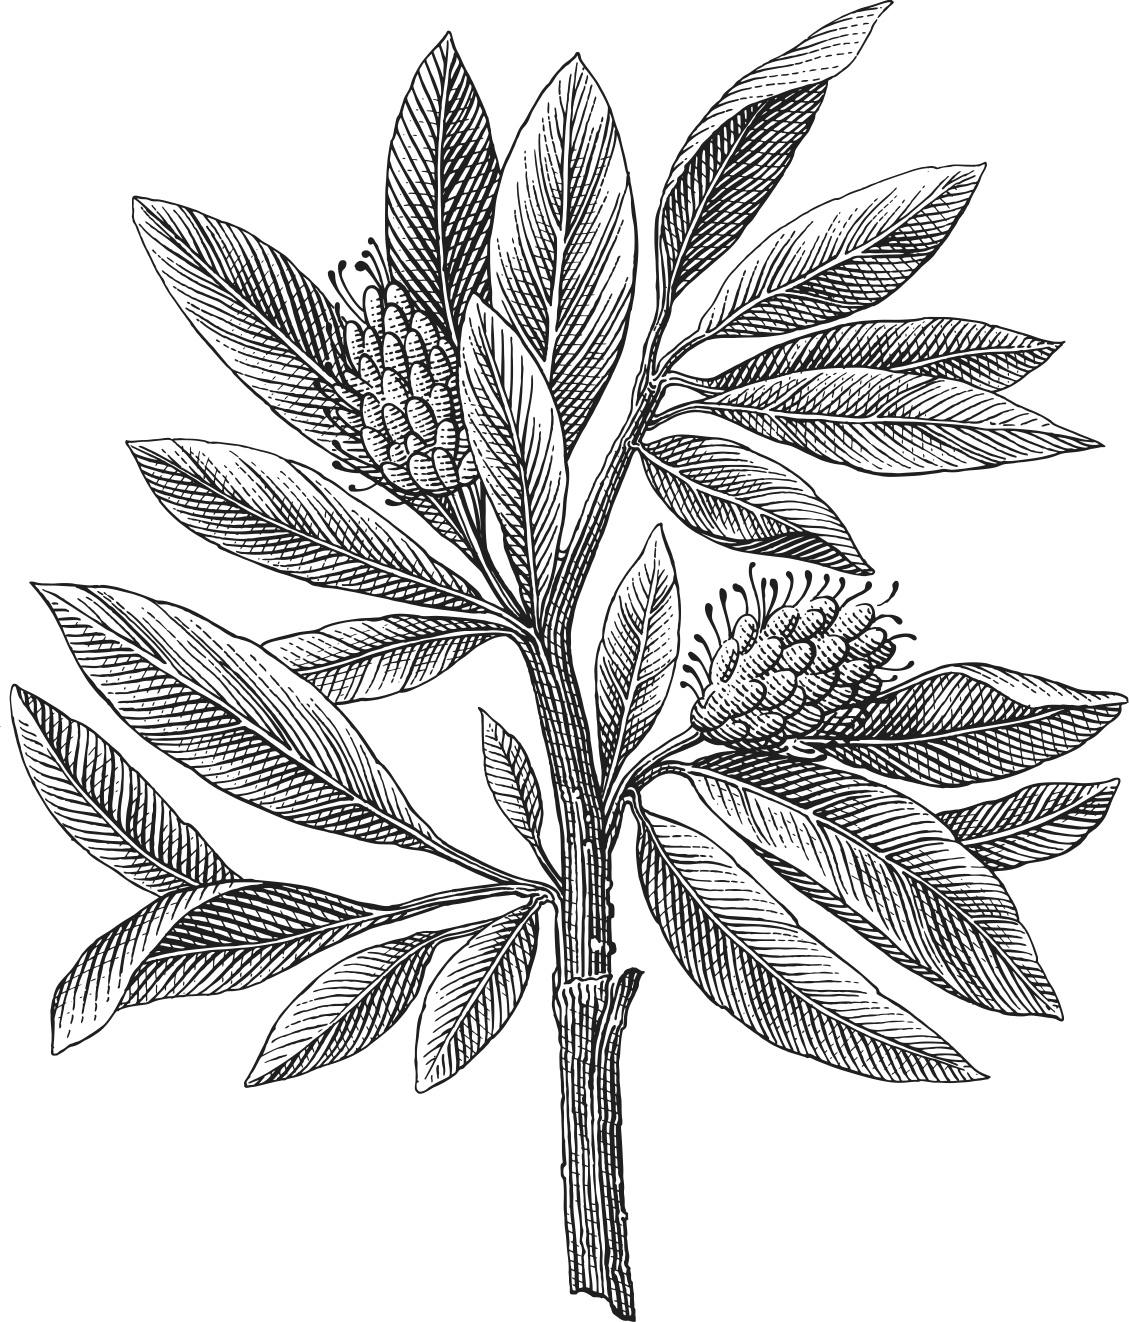
\includegraphics[keepaspectratio,scale=0.65]{lnu_etch.png} % Bakgrundsbild
    }
}
\newcommand\BackgroundPicLogo{
    \put(15,700){
    
\includegraphics[keepaspectratio,scale=0.10]{logo.png} % Logga i vänstra hörnet
    }
}

\newcommand{\horrule}[1]{\rule{\linewidth}{#1}} % Skapa hortisontell linje

\title{	\vspace{-10cm}
    \normalfont \normalsize
    \textsc{Linnaeus University} \\ [25pt] % Universitetes namn
    \horrule{0.5pt} \\[0.4cm] % Tunn linje högst upp
    \huge Seminar 2\\ % Arbetes titel
	\large \textcolor{gray}{1DV020 -- Server Administration}
    \horrule{0.5pt} \\[0.4cm] % Tunn linje längst ner
}

\author{Jacob Lindehoff} % Författarnas namn

\date{\normalsize\today} % Dagens datum

\begin{document}
  \AddToShipoutPicture*{\BackgroundPic} % Lägger in backgrundsbild på första sidan
  \AddToShipoutPicture*{\BackgroundPicLogo}
  \maketitle % Skriv ut titeln
  \noindent % Tabba inte in på första meningen

  %------------------------------------------------
  % Introduktion
  %------------------------------------------------
  \section{Introduction}
  During this seminar, we will address the following topics:
  \begin{itemize}
    \item DNS - bind
    \item DHCP
    \item Web Server
  \end{itemize}

  %------------------------------------------------
  %	Deadline
  %------------------------------------------------
  \section{Deadline}
  The seminar is on the {\color{red}25th of February 2015} and it is compulsory. If you cannot participate, it must be notified in advance and a written report of the seminar must be submitted no later than {\color{red}3 days} after the seminar. The written report should contain detailed answers to all questions in the seminar.
  \newpage

  %------------------------------------------------
  %	Seminariefrågor
  %------------------------------------------------
  \section{Seminar Questions}
  \subsection{DNS}
  \begin{enumerate}
    \begin{large}
		\item Vad är DNS och dess huvuduppgift?
		\item Vad är Forward Lookup Zone?
		\item Vad är Reverse Lookup Zone?
		\item Beskriv 10 olika toppdomäner och dess användningsområden.
		\item Utan DNS skulle inte Internet fungera:
		\begin{enumerate}[a.]
			\item Hur fungerar DNS-strukturen på Internet?
			\item Måste företagets DNS servrar vara uppkopplade mot Internets DNS servrar?
			\item Hur skiljer sig en intern DNS server från en publik?
		\end{enumerate}
		\item Hur fungerar DNS delegering och när används detta?
		\item Det finns en zon typ som är specifik för Microsofts DNS servrar, vilken är det och vad används den till?
		\begin{enumerate}[a.]
			\item	Vad är ett Glue record?
		\end{enumerate}
		\item	Hur går du till väga för att skapa redundans på en zon/domän?
		\item	Beskriv följande records:
		\begin{enumerate}[a.]
			\item CNAME
			\item PTR
			\item MX
			\item SRV
			\item NS
			\item SOA
			\item A
		\end{enumerate}
		\item Vad är Zone transfer?
		\item Vad är ROOT hints och vad används de till?
		\item Beskriv fördelar och nackdelar med DNS caching.
		\item Vad är DNS forward och hur fungerar det?
		\begin{figure}[h]
		\centering
		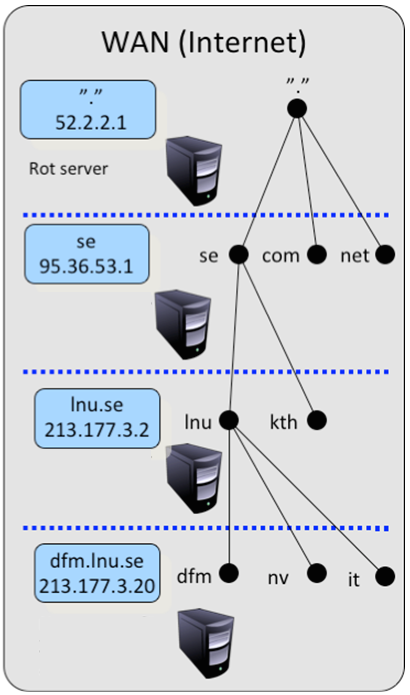
\includegraphics[width=0.5\linewidth]{./figure_1}
		\caption{Namnsservrar på Internet}
		\label{fig:figure_1}
		\end{figure}
		
		\item Låt oss säga att du har en klient som är koppla till 
		ett nätverk som har en egen DNS server som är konfigurerad med DNS forward till företagets 
		ISPs DNS server. Utgå från Figur \ref{fig:figure_1}
		\begin{enumerate}[a.]
			\item Beskriv i detalj vad som händer när klienten ställer en rekursiv DNS fråga om IP för www.dfm.lnu.se 
			\item Beskriv i detalj vad som händer när klienten ställer en iterativ DNS fråga om IP för www.dfm.lnu.se 
		\end{enumerate}
    \end{large}
    \setcounter{tmpc}{\theenumi}
  \end{enumerate}

  \subsection{DHCP}
  \begin{enumerate}
  \setcounter{enumi}{\thetmpc}	
    \begin{large}
	    \item Vad används DHCP till och på vilket sätt förenklar detta administrationen?
		\item Beskriv följande DHCP-termer:
		\begin{enumerate}[a.]
			\item Scope
			\item Exclusion range
			\item Address pool
			\item Lease
			\item Reservation
		\end{enumerate}
		\item Beskriv de olika stegen i en DHCP förfrågan?
		\item Beskriv hur DHCP kan integreras med DNS och vilka fördelar/nackdelar detta medför?
    \end{large}
    
    \setcounter{tmpc}{\theenumi}
  \end{enumerate}
  \newpage
  \subsection{Web server}
  \begin{enumerate}
  \setcounter{enumi}{\thetmpc}
    \begin{large}
    	\item Question
    \end{large}
  \end{enumerate}
\end{document}
